\documentclass{ctexart}
\usepackage{EC}
\begin{document}
\section{砷,锑,铋及其化合物}
\subsection{砷,锑,铋的卤化物}
\subsubsection{三卤化物\ce{MX3}}
所有这三种元素都能与四种卤素形成三卤化物.你可以自行查阅它们的物理性质.
\paragraph{三卤化物的反应}
这里主要介绍\ce{MF3}和\ce{MCl3}的反应.
\subparagraph{\ce{MF3}的反应}
\ce{AsF3}和\ce{SbF3}是重要的将氯化物(或者硫化物)氟化的试剂.有时在氟化过程中也伴随着氧化.一些典型的反应如下:
\begin{center}
    \ce{3F3CPCl2 + 2SbF3 -> 3F3CPF2 + 2SbCl3}\\
    \ce{3PhPCl2 + 4SbF3 -> 3PhPF4 + 2Sb + 2SbCl3}\\
    \ce{3Me2P(S)P(S)Me2 + 6SbF3 -> 6Me2PF3 + 2Sb + 2Sb2S3}
\end{center}
与\ce{SbF3}相比,\ce{AsF3}虽然是一个较弱的氟化剂,但更适合于制备高沸点氟化物,因为此时\ce{AsC13}较易蒸发除去.\ce{SbF3}则更适合制备低沸点氟化物,因为后者容易自{SbC13}中分馏出来.选择性的氟化反应也可以发生:
\begin{center}
    \ce{[PCl4][PCl6] + 2AsF3 -> [PCl4][PF6] + 2AsCl3}
\end{center}
\paragraph{三氯化物的反应}
\ce{AsCl3}和\ce{SbCl3}通常作为非水溶剂使用.此外,它们还可以用于制备各种亚砷/锑酸酯或胺基衍生物.\\
\indent \ce{BiCl3}容易水解生成\ce{BiOCl}.这是一种具有珠光白色的化合物,其板状结构的光波干涉产生类似于珍珠的珠光彩虹光反射,因此在古埃及被用于化妆品.
\subsubsection{五卤化物\ce{MX5}}
我们主要讨论\ce{As}和\ce{Sb}的五卤化物.\ce{BiF5}是具有强烈氧化性的物质,与水反应甚至生成\ce{O3},\ce{OF2}等物质.\\
\indent 除此之外,\ce{AsF5}和\ce{SbF5}可以由对应的三氟化物或单质与\ce{F2}反应得到.\\
\indent 与\ce{PCl5}和\ce{SbCl5}相比,\ce{AsCl5}稳定性较差.这也许是d区收缩的又一例子.同样地,没有\ce{BiCl5}的存在也可能是f区收缩的缘故.\\
\indent 气态的\ce{AsF5},(低温下)固态的\ce{AsCl5}和液态的\ce{SbCl5}均与\ce{PF5}相似,含有分立的三角双锥构型的分子.而液态\ce{SbF5}却有异常高的粘度,这是因为其中含有顺式桥连的\ce{\{SbF6\}}八面体的聚合链.在固体中则是\ce{[SbF5]4}四聚体.
\chemfig{SbF5}{1}{\ce{[SbF5]4}的结构}
这样的桥连结构在对应的卤素配合物中也很常见.我们将在后面讲到.
\subsection{混合卤化物和低卤化物}
\paragraph{混合卤化物}
混合三卤化物比较难生成.相反,混合五卤化物则是容易得到的.例如:
\begin{center}
    \ce{2AsF3 + 2Cl2 -> [AsCl4]+[AsF6]-}\\
    \ce{AsCl3 + SbCl5 + Cl2 -> [AsCl4]+[SbCl6]-}
\end{center}
此外还能得到一系列\ce{SbF5}四聚体的类似分子,这里就不详细介绍了.\\
\indent 向\ce{SbF5}加入少量\ce{SbCl5}可以降低其粘度并显著升高其电导率,因为破坏了\ce{F-F}桥键并且生成了\ce{[SbF5Cl]-}等配离子.
\paragraph{低卤化物}
\ce{Bi}的低卤化物有着神奇的成分和结构.将\ce{Bi}与\ce{BiCl3}的混合物加热后冷却即可得计量比为\ce{Bi6Cl7}的黑色低氯化物,其实际组成应当写作\ce{[Bi9^5+]2[BiCl5^2-][Bi2Cl8^2-]}.\\
\indent 另一个有趣的例子是\ce{HfCl4/BiCl3}氧化\ce{Bi}所得到的\ce{Bi10Hf3Cl18},其实际组成为\ce{[Bi+][Bi9^5+][HfCl6^2-]3}.
\subsubsection{卤离子配合物}
\subsection{砷,锑,铋的氧化物和含氧化合物}
\subsubsection{+3价氧化物和含氧化合物}
\paragraph{\ce{As2O3}与\ce{H3AsO3}} \ce{As2O3}是砷最重要的化合物.
\begin{substance}[\ce{As2O3}]
    砷华,又称砒霜,信石,化学式为\ce{As2O3}(依照其常见的存在形式,写作\ce{As4O6}也许更合理),为白色至淡黄色晶体,有剧毒.\ce{As2O3}可溶于水.
\end{substance}
\subparagraph{\ce{As2O3}的制备}
可以由以下几种方法制取\ce{As2O3}.
\begin{enumerate}[label=\tbf{\arabic*.},topsep=0pt,parsep=0pt,itemsep=0pt,partopsep=0pt]
    \item 在空气中燃烧砷或者一些含砷矿物.
        \begin{center}
            \ce{4As + 3O2 -> 2As2O3}\\
            \ce{2As2S3 + 9O2 -> 2As2O3 + 6SO2}\ \ \ \ \ \ce{2FeAsS + 5O2 -> Fe2O3 + As2O3 + 2SO2}
        \end{center}
    \item 水解\ce{AsCl3}.
        \begin{center}
            \ce{2AsCl3 + 3H2O -> As2O3 + 6HCl}
        \end{center}
\end{enumerate}
\subparagraph{\ce{As2O3}的结构}
气相中的\ce{As2O3}以\ce{As4O6}分子的形式存在,与\ce{P4O6}分子相似,可以冷却形成立方晶系的砷华.
\begin{figure}[H]
    \centering
    \subfigure[\ce{As4O6}的晶体结构示意图]{
        \begin{minipage}[b]{.48\linewidth}
            \centering\includegraphics[scale=0.1]{picture/As4O6-1.eps}
        \end{minipage}
    }
    \subfigure[\ce{As4O6}的晶胞沿对角线方向的投影图]{
        \begin{minipage}[b]{.48\linewidth}
            \centering\includegraphics[scale=0.1]{picture/As4O6-2.eps}
        \end{minipage}
    }\caption{立方\ce{As4O6}的晶体结构}
\end{figure}
单斜晶系的\ce{As2O3}可以由砷华在痕量水的存在下加热得到,为角锥形\ce{\{AsO3\}}单元组成的二维结构.
\chemfig{As2O3}{0.125}{单斜\ce{As2O3}的晶体结构}
\subparagraph{\ce{As2O3}的水溶液与\ce{H3AsO3}}
\indent \ce{As2O3}在水中的溶解度及存在的物种与溶液的pH值关系很大.在中性或碱性溶液中,主要的物种为亚砷酸\ce{H3AsO3}(尽管它并没有被单独分离出来).亚砷酸水溶液的\ce{^1H}核磁共振频谱中只有单一的讯号,反映其分子结构为\ce{As(OH)3},而与亚磷酸不同.
\chemfig{H3AsO3}{1}{\ce{H3AsO3}的结构}
\ce{H3AsO3}的亚砷酸是弱酸:
\begin{center}
    \ce{H3AsO3 + H2O <=> AsO(OH)2- + H3O+}\ \ \ $\text pK_{\text a1}=9.2$\\
    \ce{AsO(OH)2- + H2O <=> AsO2(OH)^2- + H3O+}\\
    \ce{AsO2(OH)^2- + H2O <=> AsO3^3- + H3O+}
\end{center}
如果以\ce{HCl}溶液作为溶剂,那么\ce{As2O3}的溶解度随\ce{HCl}浓度的增加而先减小后增大.这是因为\ce{As2O3}与\ce{HCl}反应:
\begin{center}
    \ce{As2O3 + 6HCl -> 2AsCl3 + 3H2O}
\end{center}
这恰好与\ce{AsCl3}的水解互为逆过程.
\subparagraph{亚砷酸盐和偏亚砷酸盐}
偏亚砷酸盐,例如\ce{NaAsO2}中含有多聚的链状阴离子.
\begin{figure}[H]
    \centering
    \subfigure[\ce{NaAsO2}的晶体结构示意图]{
        \begin{minipage}[b]{.48\linewidth}
            \centering\includegraphics[scale=0.1]{picture/NaAsO2-1.eps}
        \end{minipage}
    }
    \subfigure[\ce{As4O6}的晶胞沿$b$轴的投影图(去除\ce{Na}原子)]{
        \begin{minipage}[b]{.48\linewidth}
            \centering\includegraphics[scale=0.1]{picture/NaAsO2-2.eps}
        \end{minipage}
    }\caption{\ce{NaAsO2}的晶体结构及其中的\ce{\{AsO2\}}长链}
\end{figure}
\ce{Cu^{II}}的亚砷酸盐被用于绿色颜料,例如巴黎绿\ce{Cu2(OAc)(AsO3)}和舍勒绿\ce{CuHAsO3}(或其脱水物\ce{Cu2As2O5}).
\paragraph{\ce{Sb2O3}}
\ce{Sb2O3}和\ce{As2O3}一样也具有两种异构的晶型.\\
\indent 正交的\ce{Sb2O3}结构与单斜\ce{As2O3}类似,被称作\tbf{锑华};立方的\ce{Sb4O6}结构与立方\ce{As4O6}类似,被称作\tbf{方锑矿}.锑华是锑的重要矿物之一.
\paragraph{\ce{Bi2O3}与\ce{Bi(OH)3}}
\ce{Bi2O3}是\ce{Bi}最重要的化合物之一.
\begin{substance}
    三氧化二铋,即铋华,化学式为\ce{Bi2O3},为黄色晶体或粉末.
\end{substance}
\subparagraph{\ce{Bi2O3}的结构}
\ce{Bi2O3}室温下稳定存在的晶型为$\alpha$-\ce{Bi2O3},具有多聚的层状结构,其中含有变形五配位的\ce{\{BiO5\}}单元.对\ce{Bi2O3}加热可得萤石型的$\beta$-\ce{Bi2O3},其中有统计分布的\ce{O^2-}空穴.
\subparagraph{水溶液中的\ce{Bi^{III}}}
\ce{Bi(OH)3}明显应当作为一种碱性物质.它易溶于酸形成含\ce{Bi^3+}溶液,但pH升高时即生成含氧的沉淀.一般而言,在溶液中的\ce{Bi^{III}}写成\ce{BiO+}应当更加合适.\\
\indent 在生成沉淀之前,还会产生多聚的含氧阳离子.比较重要的一个是\ce{[Bi6(OH)12]^6+},其结构如下.
\chemfig{Bi6(OH)126+}{1}{\ce{[Bi6(OH)12]^6+}的结构}
\subsubsection{+5价氧化物和含氧化合物}
\paragraph{\ce{As2O5}和\ce{H3AsO4}}
五氧化二砷是很早便知道的一种氧化物
\subparagraph{\ce{As2O5}}
五氧化二砷\ce{As2O5}的结构与\ce{P4O10}并不相同,其中含有等量的\ce{\{AsO6\}}八面体和\ce{\{AsO4\}}四面体,以共用角的方式形成管状孔穴结构.
\chemfig{As2O5}{0.125}{\ce{As2O5}的晶体结构示意图}
\begin{figure}[H]
    \centering
    \subfigure{
        \begin{minipage}[b]{.48\linewidth}
            \centering\includegraphics[scale=0.12]{picture/As2O5-1.eps}
        \end{minipage}
    }
    \subfigure{
        \begin{minipage}[b]{.48\linewidth}
            \centering\includegraphics[scale=0.12]{picture/As2O5-2.eps}
        \end{minipage}
    }\caption{\ce{As2O5}中的管状空穴结构}
\end{figure}
这也解释了\ce{As2O5}中只有一半的\ce{As}能被\ce{Sb}(六配位)或\ce{P}四配位替换的现象.\\
\indent \ce{As2O5}可由\ce{As2O3}与加压的\ce{O2}反应得到,也可以由\ce{H3AsO4}脱水得到.\ce{As2O5}具有较强的氧化性,它可以和\ce{HCl}反应生成\ce{Cl2}:
\begin{center}
    \ce{As2O5 + 10HCl -> 2AsCl3 + 5H2O + 2Cl2}
\end{center}
\subparagraph{\ce{H3AsO4}}
砷酸\ce{H3AsO4}可以由浓\ce{HNO3}氧化\ce{As2O3}制取:
\begin{center}
    \ce{As2O3 + 4HNO3 + H2O -> 2H3AsO4 + 4NO2}
\end{center}
与磷酸一样,\ce{H3AsO4}也是三元酸.
\begin{center}
    \ce{H3AsO4 + H2O <=> H2AsO4- + H3O+}\ \ \ $\text pK_{\text{a}1}=2.21$\\
    \ce{H2AsO4- + H2O <=> HAsO4^2- + H3O+}\ \ \ $\text pK_{\text{a}2}=6.96$\\
    \ce{HAsO4^2- + H2O <=> AsO4^3- + H3O+}\ \ \ $\text pK_{\text{a}1}=11.50$
\end{center}
\ce{H3AsO4}的氧化性不强,但强于\ce{H3PO4}:
\begin{center}
    \ce{H3AsO4(aq) + 2H+(aq) + 2e- -> H3AsO3(aq) + H2O(l)}\ \ \ $\varphi^\ominus=0.575\V$
\end{center}
在弱酸性缓冲溶液(例如硼砂-硼酸或\ce{H2PO4-}-\ce{HPO4^2-})中,\ce{As^{III}}能被\ce{I2}定量氧化至\ce{As^{V}}.这可以作为测定\ce{As}含量的方法.
\begin{center}
    \ce{H3AsO3 + I2 + H2O + HPO4^2- -> 2I- + H2PO4- + H2AsO4-}
\end{center}
\paragraph{\ce{Sb2O5}和\ce{H3SbO4}}
\ce{Sb2O5}可以由\ce{SbCl5}水解后脱水得到,但并不稳定.而\ce{H3SbO4}的性质则与\ce{H3AsO4}相似.
\paragraph{\ce{Bi^{V}}酸盐}
尚未明确地指出\ce{Bi2O5}的存在.不过,铋酸盐已经被广泛地用作氧化剂,这其中最重要的就是\ce{NaBiO3}.
\begin{substance}[\ce{NaBiO3}]
    铋酸钠,化学式为\ce{NaBiO3},为黄色至棕黄色粉末,不溶于水.
\end{substance}
如有必要,生成\ce{NaBiO3}的反应需要记得标注沉淀符号.\ce{NaBiO3}参与反应时离子方程式不可拆写.\\
\indent \ce{NaBiO3}可以由以下方法制备:
\begin{center}
    \ce{Bi2O3 + 6NaOH + 2Br2 -> 2NaBiO3 + 4NaBr + 3H2O}\\
    \ce{Na2O + Bi2O3 + O2 -> 2NaBiO3}
\end{center}
作为一种强氧化剂,\ce{NaBiO3}在潮湿的环境下会缓慢分解:
\begin{center}
    \ce{2NaBiO3 + H2O -> 2NaOH + Bi2O3 + O2}
\end{center}
在酸中分解得更快.与\ce{HCl}反应则会氧化\ce{Cl-}而产生\ce{Cl2}.\\
\indent \ce{NaBiO3}可以定性和定量地检测\ce{Mn}.在酸性条件下,\ce{NaBiO3}可以将\ce{Mn^2+}定量氧化为\ce{MnO4-},出现标志性的紫色,且容易通过分光光度法定量检测.
\subsection{砷,锑,铋的硫化物}
\subsubsection{砷的硫化物}
\begin{substance}[\ce{As4S4}]
    雄黄,又称鸡冠石,化学式为\ce{As4S4},为不溶于水的橙红色晶体.\ce{As4S4}的熔点为$320\tc$,但非常容易升华.
\end{substance}
\begin{substance}[\ce{As2S3}]
    雌黄\footnotemark,又称石黄,化学式为\ce{As2S3},为不溶于水的黄色晶体.
\end{substance}\footnotetext{所谓信口雌黄,就是用雌黄涂抹黄色的纸以达到修改文字的目的.}
\paragraph{各种硫化物的结构}
雌黄晶体和\ce{As2O3}一样具有二维层状结构.\\
\indent 雄黄晶体中含有分立的\ce{As4S4}分子.正如\ce{P4S4}一样,\ce{As4S4}也有两种异构体.雄黄中的\ce{As4S4}采取对称的$D_{2\text d}$形式,其结构与\ce{S4N4}正好相反,所有\ce{S}原子(接近)共平面,\ce{As}原子分立两侧.\\
\indent 当用\ce{AS4S3}在\ce{S}的\ce{CS2}溶液加热以制取\ce{As4S4}时,偶尔能得到较少的针状桔红色晶体\ce{As4S5}.它的结构与\ce{P4S5}有所不同,仅有一根\ce{As-As}键,并且没有端基\ce{S}原子.这也是\ce{As}较难被氧化至\ce{As^{V}}的体现.
\paragraph{雄黄与雌黄的反应}
\ce{As2S3}在空气中燃烧即生成\ce{As2O3}与\ce{SO2}.\ce{As2S3}与\ce{Cl2}反应则生成\ce{AsCl3}与\ce{S2Cl2}.
\begin{center}
    \ce{2As2S3 + 9O2 -> 2As2O3 + 6SO2}\\
    \ce{2As2S3 + 9Cl2 -> 4AsCl3 + 3S2Cl2}
\end{center}
\ce{As2S3}不溶于水,但可以溶于碱性溶液或碱金属硫化物的溶液.
\begin{center}
    \ce{As2S3 + 2Na2S -> 2Na2AsS2}
\end{center}
它也可以在多硫化物的溶液中生成硫代砷酸盐\ce{M3AsS4},产物非常难溶.\\
\indent 当\ce{As2S3}用沸腾的\ce{Na2CO3}溶液处理时可以得到\ce{As4S4};或者采用黄铁矿与砷黄铁矿共热的办法制取.
\begin{center}
    \ce{6As2S3 + 6Na2CO3 -> 3As4S4 + 4Na2S + 2Na2SO3 + 6CO2}\\
    \ce{4FeS2 + 4FeAsS -> 8FeS + As4S4}
\end{center}
在自然界中,雄黄会自发地转化为雌黄(即雄黄千年变雌黄).这可能是由于空气中的\ce{O2}将\ce{As4S4}部分氧化所致.
\begin{center}
    \ce{3As4S4 + 3O2 -> 4As2S3 + 2As2O3}
\end{center}

\subsubsection{锑,铋的硫化物}
在这些物质中最重要的是\ce{Sb2S3}.
\begin{substance}[\ce{Sb2S3}]
    三硫化二锑,化学式为\ce{Sb2S3},黄红色无定形粉末或深灰色晶体.
\end{substance}
辉锑矿的成分即为\ce{Sb2S3}.
\subsection{\ce{M-M}键化合物与原子簇}
\subsubsection{\ce{M2R4}型化合物}
联胂\ce{As2H4}是亚砷酸盐的碱性溶液以\ce{BH4-}还原并酸化以使其形成\ce{AsH3}时产生的少量副产品,也可以由\ce{AsH3}放电得到.\ce{As2H4}是极不稳定的液体,室温下即分解为成分复杂的氢化物.将\ce{H}替换为有机基团的类似物则稳定一些.例如:
\begin{center}
    \ce{2Ma2AsI + 2Li ->T[\ce{THF}] As2Me4 + 2LiI}
\end{center}
产物双甲胂是剧毒且有令人厌恶的气味的气体.\\
\indent \ce{Sb}和\ce{Bi}的类似物则更不稳定.
\subsubsection{环状多聚物与异核原子簇}
环多聚胂\ce{(RAs)_n}可以由有机胂的二卤化物或胂酸还原而制备,例如
\begin{center}
    \ce{6PhAsCl2 + 12Na ->T[\ce{Et2O}] (PhAs)6 + 12NaCl}\\
    \ce{2PhAsI2 + 2Hg -> PhIAsAsIPh + Hg2I2}\ \ \ \ \ \ce{3PhIAsAsIPh + 6Hg -> (PhAs)6 + 3Hg2I2}\\
    \ce{5PhAsO(OH)2 + 5H3PO2 -> (PhAs)5 + 5H3PO4 + 5H2O}
\end{center}
其它基团,例如\ce{Me,Et,CF3}等等的类似物也可以由这些方法制备.一个特殊的例子如下所示:
\chemfig{As3C5H9}{1}{\ce{MeC(CH2As)3}的笼状结构}
其中保留了\ce{[As3]}环状结构.\\
\indent \ce{AsR3}可以作为良好的配体,这些聚合物亦如此.例如,\ce{(MeAs)5}与\ce{Cr(CO)6}反应可以生成\ce{Cr(CO)3(As5Me5)},其结构示意如下:
\chemfig{Cr(CO)3(As5Me5)}{1}{\ce{Cr(CO)3(As5Me5)}的结构}
其余的更复杂的类似物可以自行查阅资料.\\
\indent 另外一件比较重要的事实是\ce{As}和\ce{Co(CO)3}基团是等电子的.这意味着这两者可以在\ce{[As4]}簇的基础上进行替换,形成诸如\ce{As3Co(CO)3},\ce{As2Co2(CO6)}等笼状簇合物.正因如此,\ce{Co2+}在适合的配体存在下可与\ce{As4}反应生成与\ce{[Bi5]^2+}类似的簇合离子,其结构如下图所示.
\chemfig{As3Co2L22+}{1}{\ce{[As3Co2L2]2+}的结构示意图}
将\ce{Co}替换为\ce{Ni},或进行单电子氧化/还原,即可得到电子数不同的,可能具有顺磁性的类似物.\\
\indent 对于\ce{Sb}而言,可以得到更大的原子簇,例如\ce{Sb4\{Co(CO)3\}4},其结构如下所示,是一个变形的立方体.
\chemfig{Sb4Co4(CO)12}{1}{\ce{Sb4\{Co(CO)3\}4}的结构}
\subsubsection{同核阴离子簇}
碱土金属的磷化物\ce{M3P14}中含有\ce{[P7]^3-}离子,它与\ce{P4S3}是等电子体.类似的\ce{[As7]^3-}和\ce{[Sb7]^3-}也是存在的.\ce{[As7]^3-}还可以与\ce{TMSCl}发生取代反应生成对应的中性分子.
\chemfig{As73-}{1}{\ce{[As7]^3-}的立体结构}
用\ce{KAs2}与crypt在乙二胺中反应可以得到具有近$D_3$对称性的\ce{[As11]^3-},其结构如下.
\chemfig{As113-}{1}{\ce{[As11]^3-}的立体结构}
\subsubsection{同核阳离子簇}
铋可以形成多种同核阳离子簇.现在将其结构列举如下.
\begin{figure}[H]
    \centering
    \subfigure[\ce{[Bi5]^3+}]{
        \begin{minipage}[b]{.3\linewidth}
            \centering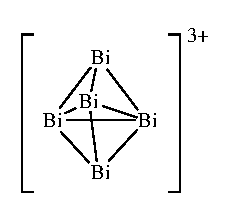
\includegraphics{picture/Bi53+.eps}
        \end{minipage}
    }
    \subfigure[\ce{[Bi8]^2+}]{
        \begin{minipage}[b]{.3\linewidth}
            \centering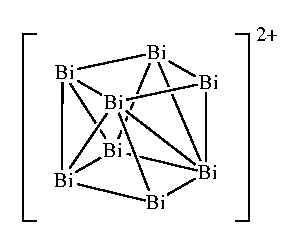
\includegraphics{picture/Bi82+.eps}
        \end{minipage}
    }
    \subfigure[\ce{[Bi9]^5+}]{
        \begin{minipage}[b]{.3\linewidth}
            \centering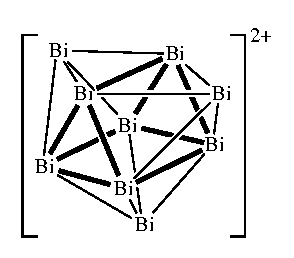
\includegraphics{picture/Bi95+.eps}
        \end{minipage}
    }\caption{\ce{[Bi_n]^m+}阳离子簇的结构}
\end{figure}
\ce{[Bi5]^3+}和\ce{[Bi8]^2+}可以由以下方法制备.
\begin{center}
    \ce{BiCl3 + 4Bi + 4AlCl3 ->T[\ce{NaAlCl4}] [Bi5][AlCl4]3}\\
    \ce{2BiCl3 + 14Bi + 4AlCl3 ->T[\ce{NaAlCl4}] 2[Bi8][AlCl4]2}\\
    \ce{10Bi + 9AsF5 ->T[\ce{SO2}] 2[Bi5][AsF6]3.2SO2 + 3AsF3}
\end{center}

\end{document}